\iffalse
To find the condition number, I have created a small function in the "Q0016.py" file to find the inverse of $A$ and multiply the norms of $A$ and $A^{-1}$.
\begin{figure}[ht]
  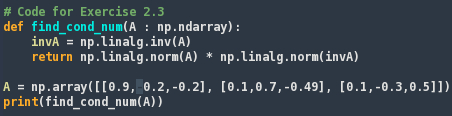
\includegraphics[width=1\linewidth]{find_cond_num}
  \caption{Function used to calculate the condition number of $A$}
\end{figure}

With this we find that the matrix $A$ has a condition number of $6.4072$. \\
I have been unable to solve the rest of this and would like to know where to go from here. I am unsure as to how the condition number of $A$ can be used to solve this. \\
I realise that $r = b - \tilde{b}$ is equal to some constant multiplied by our error. I am unsure however what $r$ is, since normally it is defined as the simple root so that $f'(r) \neq 0$, but here is defined as part of the linear equation system $A$.
\fi
To compute the condition number of $A$, we use the following formula:
$$
_K(A) = ||A|| \cdot ||A^{-1}||
$$
With this, we get the condition number of $A$ to equal $6.407$. We use the theorem on pg. 193 of the textbook:
\begin{align*}
  \frac{1}{_K(A)}\frac{||r||}{||b||} &\leq \frac{||e||}{||x||} \leq _K(A) \frac{||r||}{||b||}
\end{align*}
Since $||r|| = \mathcal{E} ||b||$, we can rewrite to the following:
\begin{align*}
  \frac{\mathcal{E}}{_K(A)} &\leq \frac{||e||}{||x||} \leq _K(A)\mathcal{E}
\end{align*}
Since $\frac{||e||}{||x||}$ is the relative error, we can bound it thus:
\begin{align*}
  \frac{\mathcal{E}}{6.407} &\leq \frac{||e||}{||x||} \leq 6.407\mathcal{E}
\end{align*}
